\section{Open problems in applications of mechanistic interpretability}
\label{sec:open-problems-applications}

Ultimately, we need mechanistic interpretability methods that enable us to solve concrete scientific and engineering problems (\Cref{fig:applications}). While predicting the impact of fundamental science in advance is difficult, having concrete goals in mind during research is usually beneficial. We want mechanistic interpretability methods to help us achieve various outcomes, such as monitoring and auditing AI systems more effectively (\Cref{subsec:monitoring-and-auditing}), controlling of AI system behavior more precisely (\Cref{subsec:better-control}), predicting AI system outcomes more accurately (\Cref{subsec:better-predictions}), enhancing AI system capabilities (\Cref{subsec:capabilities}), and extracting knowledge from AI systems (\Cref{subsec:microscope-ai}). We should also anticipate that mechanistic interpretability will uncover “unknown problems” present in systems, revealing that the true realm of challenges and possibilities is greater than what we currently perceive it to be.

As highlighted in the previous section, progress in mechanistic interpretability methods is multifaceted. Each axis of methodological advancement leads to varying degrees of progress toward different goals. Before we discuss open questions in its applications, we identify distinct axes of methodological progress that lead to different amounts of progress toward different goals. 


\subsection{Axes of mechanistic interpretability progress.}
\label{subsec:axes}

\textbf{Decomposition vs. description of network components}: Improvements in network decomposition versus component description methods offer varying benefits for different goals. Decomposition methods vary in their efficacy at carving networks at the joints of their generalization structure, while description methods can yield descriptions that vary in depth. Deeper descriptions of a component are typically more causal or mechanistic, whereas shallower descriptions may rely more on correlations and only connect to inputs or outputs without referencing intermediate causes or effects (\Cref{fig:descriptions}. Deeper descriptions thus attempt to explain more about how the component interacts with other components within the network's algorithm. Certain goals can be achieved with minimal or no progress in decomposition or description, while others may demand substantial progress.

\textbf{Extent of network decomposition or description}: The extent of network decomposition or description needed may vary depending on the goal. Certain goals only require an understanding of specific network components (such as an individual features or a circuit), while others might require enumerating or understanding of larger circuits or the entire model (as in `enumerative safety').

\textbf{Extent of task distribution analyzed}: The scope of task distribution analysis also depends on the intended goal. For instance, monitoring a model for a single kind of behavior might only require decomposing or understanding the model only over a narrow task distribution, while others, such as formal verification, might demand understanding over the entire distribution of tasks.

\textbf{Mechanistic understanding post vs. during training}: Understanding the mechanisms of a fixed model might suffice for some goals, but more ambitious goals might require an understanding of not only the models' mechanisms, but also how they change during the learning process.

In this section, we'll discuss how mechanistic interpretability has been used or could be leveraged to further the field's various goals. We'll assess the progress made thus far, and identify the advancements along different axes of methodological progress that will be most crucial to success.


\begin{figure}[h]
    \centering
    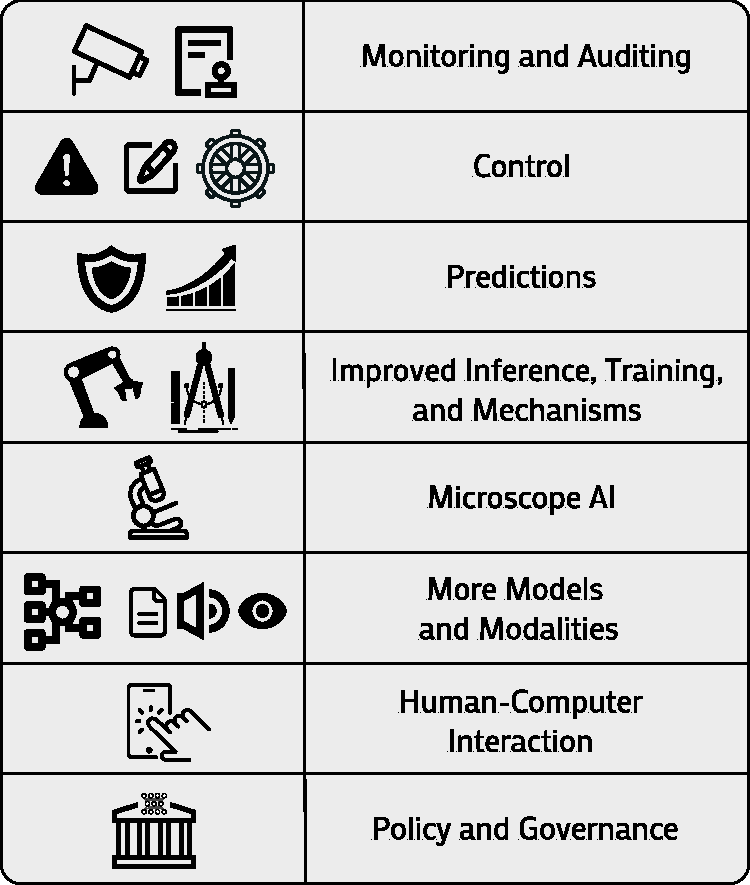
\includegraphics[width=0.8\textwidth]{figures/applications.pdf}
    \caption{A summary of problem areas for applications of mechanistic interpretability.}
    \label{fig:applications}
\end{figure}


\subsection{Using mechanistic interpretability for better monitoring and auditing of AI systems for potentially unsafe cognition}
\label{subsec:monitoring-and-auditing}

\subsubsection{Mechanistic interpretability-based evaluations could help us detect unsafe or unethical AI cognition}
\label{par:interp-evals}

Currently, we rely on “black box” evaluations to understand a model's capabilities, but studying input-output behavior alone may not reveal all dangerous behaviors. Such behaviors include deceiving users \citep{park2023aideceptionsurveyexamples, ward2023honesty, scheurer2024largelanguagemodelsstrategically, meinke2024frontiermodelscapableincontext}; for instance, by intentionally underperforming on evaluations (“sandbagging”, \citet{vanderweij2024aisandbagginglanguagemodels}), leveraging situational awareness \citep{laine2024me}; or giving dishonest responses tailored to match the user’s beliefs (“sycophancy”; \citet{sharma2023understandingsycophancylanguagemodels}). Interpretability techniques could be used to uncover the mechanisms underlying these potentially harmful behaviors and thus help to detect and characterize them. This becomes increasingly important as the capabilities of models increases, especially when using training methods that incentivize models to feign particular properties for the purpose of passing evaluation. 

Using interpretability methods to identify internal signs of concern (also known as “white-box” evaluations \citep{Casper_2024} or “understanding-based” evaluations \citep{hubinger2023towards}) is therefore an important problem. White-box evaluation methods could serve as tools to detect potential biases that arise when models learn to use spurious correlations \citep{gandelsman2024interpretingclipsimagerepresentation, Caspar_2022_featurelevel, Abid_2022_counterfactualExplanations}. However, human judgment might be required to determine which features are `supposed' to be relevant to the task \citep{marks2024sparsefeaturecircuitsdiscovering, Kim_2018_Activation, Goyal_2022}.

Despite current shortcomings in decomposition and description, white-box evaluations are likely feasible today. Even shallow, correlation-based descriptions could signal potentially concerning cognition. For example, developing new methods that reliably distinguish between features that merely recognize deceptive behavior vs. mechanisms that cause deceptive behavior may be challenging. However, a correlation-based method that flags both can facilitate catching the latter. To be useful, it may not even be necessary to decompose or describe the entire network; having descriptions for components that are used on concerning subdistributions of model behavior might suffice. For instance, imperfect interpretability methods may help evaluators develop hypotheses about how models will behave, thus guiding further inquiry. Meanwhile, recent work proposes incorporating SDL (\Cref{par:sdl}) into safety cases for advanced AI systems. By monitoring internal representations, it could aid in detecting potential sabotage or deceptive behavior before deployment \citep{grosse2024three}. While such approaches show promise, they have difficulty in validating whether learned features capture all concerning patterns of reasoning reliably.

Evaluations for unsafe cognition may be a particularly important use case as it plays well to the comparative advantages of mechanistic interpretability relative to the other areas of machine learning. The majority of other areas of machine learning already focus on controlling or steering the behavior of AI systems to alter input-output behavior. It is therefore unclear that this is to mechanistic interpretability's comparative advantage. On the other hand, interpretability is perhaps the only research area that attempts to understand the mechanisms of model cognition. This implies that it might be particularly fruitful for interpretability researchers to tackle problems that become easier to solve through improving such understanding: auditing for unsafe cognition, debugging unexpected behavior, and monitoring systems in deployment.

\parasection{Enabling real time monitoring of AI systems for potentially unsafe cognition}
\label{par:monitoring}

Beyond white-box evaluations, interpretability has further applications in monitoring. For instance, internals could be used to passively monitor the system during deployment, much like content moderation systems currently in use today. Alternatively, internals could be used to flag when a model takes an action for abnormal reasons even in absence of satisfactory descriptions (\Cref{subsec:reverse-engineering-step-2}), known as “mechanistic anomaly detection” \citep{Christiano_2022_MAD,Johnston_2024_MAD}, which may be a sign of suspicious behavior. Mechanistic anomaly detection primarily requires progress in decomposition methods (\Cref{subsec:reverse-engineering-step-1}) as it is necessary to be confident about what constitutes an individual mechanism within the network. Current SDL methods identify active latents, but not active mechanisms, which are implemented by network parameters. It may not be necessary to have deep descriptions of the function of individual mechanisms as long as anomalies can be detected.

\parasection{Improving our ability to red-team AI systems and elicit unsafe outputs}
\label{par:red-teaming}

Beyond white-box evaluations, leveraging interpretability could improve our ability to conduct adversarial attacks, red-team, or jailbreak AI systems \citep{Casper_2024}. This process is beneficial as it exhibits failure modes models may display in the wild, when facing adversarial pressure from wide deployment or malicious actors, thereby enabling developers to effectively preempt and address them. Furthermore, it may form a significant element of safety cases \citep{clymer2024safetycasesjustifysafety, balesni2024evaluationsbasedsafetycasesai,grosse2024three,goemans2024safetycasetemplatefrontier} for AI systems, by providing assurances of form: We tried hard to red-team the system, yet failed to exhibit concerning behavior despite having \textit{more} affordances than users may have. One reasonable assumption is that developers may have white-box access to models, while users may not. Although many existing red-teaming methods \citep{perez2022redteaminglanguagemodels,zou2023universaltransferableadversarialattacks} already require gradient access, we could additionally leverage interpretability insights to accelerate red-teaming. For instance, \citet{arditi2024refusallanguagemodelsmediated} discovered a universal “refusal direction” in chat-finetuned language models, which is causally important for models engaging in the behavior of refusing harmful requests. \citet{lin2024understandingjailbreakattacksllms} used this to red-team models by optimizing for inputs that minimize the projection of the residual stream onto this direction during the forward pass. This approach may be more efficient than optimizing over the whole model, as previous methods did \citep{zou2023universaltransferableadversarialattacks}. Mechanistic interpretability techniques also promise to improve our ability to attribute model outputs to their corresponding inputs \cref{par:activation-causes}. This could enhance human red-teamers' ability to find key input features responsible for bad behavior in models, thus speeding up iteration cycles. Though such approaches are possible today with only feature-based understanding, they might improve with more crisp mechanism-based understanding.

\subsubsection{Using mechanistic interpretability for better control of AI system behavior}
\label{subsec:better-control}

Ensuring the safe deployment of AI first requires effective control over their behavior. Currently, the techniques used for this purpose are mostly unrelated to interpretability (e.g. \citet{christiano2023deepreinforcementlearninghuman}; \citet{rafailov2024directpreferenceoptimizationlanguage}; inter alia), but sometimes inspired by it (\citet{panickssery2024steeringllama2contrastive}, \citet{zou2024improvingalignmentrobustnesscircuit}, \citet{kirch2024featurespromptsjailbreakllms}; inter alia). Mechanistic interpretability could assist in interpreting  \citep{lee2024mechanisticunderstandingalignmentalgorithms} and improving \citep{conmy2024activation} these control methods, or in developing new ones. In this section, we outline interpretability-inspired control methods, and envision future possibilities with further progress in interpretability methods.


One new control method derived from mechanistic interpretability insights is \textbf{activation steering} (a.k.a. activation addition). A fixed activation vector, hypothesized to linearly represent a model concept, is added to an intermediate activation of a model at inference time \citep{2024inferencetimeinterventionelicitingtruthful, turner2024steeringlanguagemodelsactivation,zou2023representationengineeringtopdownapproach,panickssery2024steeringllama2contrastive}. \citet{turner2024steeringlanguagemodelsactivation} introduced activation steering, directly inspired by the Linear Representation Hypothesis (discussed in \Cref{par:sdl}). This technique results from the hypothesis, and its success can be thought of as evidence for the hypothesis. Moderate success can be achieved in steering using basic decomposition and description methods. Mechanistic interpretability decomposition methods enable the steering of models toward a narrower range of behaviors with fewer side effects \citep{chalnev2024improvingsteeringvectorstargeting}. Advancements in mechanistic interpretability methods are likely to result in improved steering capabilities, such as activating entire mechanisms instead of individual features.

\textbf{Machine unlearning} was originally defined as the problem of scrubbing the influence of particular data points on a trained machine learning model \citep{Cao_2015_MachineUnlearning}. In the context of modern generative models, machine unlearning is more broadly defined as removing particular undesirable knowledge or capabilities ('unlearning targets') from models, while preserving model performance on tasks involving non-targets \citep{liu2024rethinkingmachineunlearninglarge}. Targets for unlearning that are of particular interest include sensitive private or copyrighted data, model biases \citep{liu2024machineunlearninggenerativeai}, and hazardous knowledge that could be misused by malicious actors \citep{li2024wmdp}; for instance, information regarding the creation of bioweapons. A better understanding of how knowledge or capabilities are implemented within model internals can help in the development of new techniques for machine unlearning \citep{belrose2023leaceperfectlinearconcept,zou2024improvingalignmentrobustnesscircuit, guo2024robust,pochinkov2024dissectinglanguagemodelsmachine, ashuach2024revsunlearningsensitiveinformation}, as well as to better evaluate unlearning efficacy through white-box, non-behavioral, techniques \citep{lynch2024methodsevaluaterobustunlearning,deeb2024unlearningmethodsremoveinformation,hong2024intrinsicevaluationunlearningusing}. Thus far, mechanistic interpretability methods that modify intermediate activations (but not weights) for unlearning have yet to yield competitive results \citep{farrell2024applyingsparseautoencodersunlearn}.

Unlearning falls under the broader aim of \textbf{model (knowledge) editing}, which seeks to make precise modifications to a machine learning model that incorporates specific knowledge with desirable generalization properties, while minimizing the impact on other knowledge \citep{wang2023knowledgeeditinglargelanguage}. By attempting to carve neural networks at their joints, mechanistic interpretability could improve our ability to make interventions on knowledge with few side effects. \citet{meng2023locatingeditingfactualassociations} make initial progress toward interpretability-based model editing with their ROME technique. However, \citet{Thibodeau_2022} and \citet{hase2023doeslocalizationinformediting} highlight flaws in the technique, indicating that mechanistic interpretability has not yet found appropriate model components to intervene on (\Cref{subsec:reverse-engineering-step-1}). With better comprehension of neural networks, we should anticipate more surgical model editing techniques in the future.

Editing any given capability or piece of knowledge presents a greater challenge than deleting them. Meaningful progress in unlearning and editing methods may depend on improved network decomposition methods, as it would require isolating the individual mechanisms that correspond to specific knowledge or capabilities. Progress in mechanistic interpretability may elucidate the structure of knowledge and capabilities in AI models, leading to a better understanding of what kinds of model edits possibilities are realistic in future. Knowledge and capabilities could, in fact, be part of large mechanisms that overlap with each other, making it challenging to isolate them into discrete components. For mechanistic interpretability to effectively guide editing, strong description methods will be necessary to understand how to modify specific targets without affecting others.

Finally, mechanistic interpretability may provide tools to rigorously \textbf{understand how finetuning alters models}. This may assist in debugging instances in which finetuning leads to undesired and spurious effects \citep{casper2023openproblemsfundamentallimitations}. Recent work \citep{jain2024mechanisticallyanalyzingeffectsfinetuning, prakash2024finetuningenhancesexistingmechanisms, lee2024mechanisticunderstandingalignmentalgorithms} suggests that existing finetuning methodologies primarily make shallow edits to existing model representations and circuitry. Importantly, this suggests that harmlessness training (which trains models to refuse to answer harmful requests) may be cheaply undone. Empirical evidence supports this claim, both with further finetuning \citep{gade2024badllamacheaplyremovingsafety,lermen2024lorafinetuningefficientlyundoes}, as well as with causal interventions on the forward pass \citep{arditi2024refusallanguagemodelsmediated}. Separately, localizing knowledge and capabilities within models may improve the sample efficiency of finetuning, by selectively modifying only relevant parameters (as in, e.g. \citet{wu2024reftrepresentationfinetuninglanguage}). Further advancement in tools for comparing feature-level differences between models (such as \citet{lindsey2024crosscoders}) may accelerate our ability to debug finetuning or other control methods \citep{bricken2024stage}. Mechanistic interpretability work has thus yielded several insights into how finetuning changes models and how to improve it, and may provide further insights and improvements in the future. 

\subsection{Using mechanistic interpretability for better predictions about AI systems}
\label{subsec:better-predictions}

Accurately predicting model behavior in new scenarios or regimes is difficult (arguably impossible) without understanding model internals. Interpretability could hopefully facilitate two kinds of predictions:
\begin{itemize}
    \item Predicting model behavior in novel situations
    \item Predicting capabilities that arise during training or finetuning
\end{itemize}

\subsubsection{Predicting behavior in novel situations}
\label{subsubsec:predicting-behavior-in-novel-situations}

In order to determine whether an AI system may potentially underperform poorly or pose a safety risk in new situations, the ability to predict its behavior in untested settings is imperative. A model's behavior, which may only become apparent in unforeseen circumstances, cannot be fully captured by its performance on a finite set of behavioral evaluations.

By understanding the mechanisms of jailbreaking, we can anticipate the means through which a user might bypass existing safeguards \citep{lee2024mechanisticunderstandingalignmentalgorithms,arditi2024refusallanguagemodelsmediated}. Similarly, if models have “trojans”, backdoors \citep{hubinger2024sleeperagentstrainingdeceptive}, adversarial examples, or biases, comprehending a model's internal mechanisms could improve our ability to predict when models will display undesirable behavior, even if these scenarios were not encountered during standard training or behavioral evaluations. \citet{casper2023redteamingdeepneural} benchmark feature synthesis tools through their ability to aid developers in identifying trojans, while interpretability assisted in identifying cases of adversarial examples 
\citep{gandelsman2024interpretingsecondordereffectsneurons, Mu_2020_Advances,Wang_2022_Circuits, Kissane_Conmy_Nanda_2024}, and SDL was used to uncover biases based on spurious correlations in an LLM-based classifier \citep{marks2024sparsefeaturecircuitsdiscovering}. Beyond specific failures, interpretability methods can also be used to gain a broader understanding of network behavior. For example, prior work identified signatures in model internals that predict a model’s likelihood of hallucinating \citep{yu2024mechanisticunderstandingmitigationlanguage} or its knowledge of particular facts \citep{gottesman2024estimatingknowledgelargelanguage}.

Generally, being able to predict an AI system's behavior in advance is more challenging -- but also more desirable -- than merely being able to monitor its behavior and cognition. Mechanistic interpretability could allow us to make a certain type of claim, namely, “there exists no mechanisms that would cause the model to deliberately behave undesirably” \citep{olah2023interpretability}. For a strong version of this claim, substantial progress in both decomposition and description methods is necessary. However, weaker versions of the claim, addressing specific undesirable behaviors, might be more feasible with near-term methods. For instance, if it is possible to decompose networks and identify all components, even basic description methods might let us recognize that there are no mechanisms relating to bioweapons or illicit substances within the network, thus letting us predict that models are probably not capable of instructing users how to fabricate bioweapons or illicit substances (a possibility sometimes referred to as “enumerative safety” \citep{elhage2021mathematical, olah2023interpretability}). As AI systems become increasingly agentic, claims about even more general behavior may be possible. Understanding their values or goals (or, less anthropomorphically, `the internal mechanisms that determine their action plans and actions') should enable us to better predict their behavior across a broad range of contexts \citep{colognese2023high}.

When deploying AI in high-stakes scenarios, rigorous and reliable predictions are necessary, much like those demanded of safety-critical software applications. Sometimes, such software is formally verified, thereby ensuring certain safety-critical aspects of its behavior are guaranteed, since its compliance with specific properties is mathematically proven. In the context of mechanistic interpretability, the equivalent would be formal verification of AI systems \citep{dalrymple2024guaranteedsafeaiframework,tegmark2023provablysafesystemspath, critch2020airesearchconsiderationshuman}: mathematically proving that an AI system's behavior will satisfy a desired property on any input in a given distribution. Formal verification of AI systems remains an unresolved issue at present. The level of understanding of AI necessary to enable formal verification of large, general AI systems for nontrivial properties is well beyond the current capabilities of mechanistic interpretability. However, some recent studies using toy models provide a glimpse into what solving formal verification of AI might look like. Approaches inspired by mechanistic interpretability have been used to prove accuracy bounds on a single-layer transformer trained on a synthetic task, albeit with great difficulty \citep{gross2024compactproofsmodelperformance}. Program synthesis through mechanistic analysis offers an alternative approach by converting simple trained neural networks into more interpretable, controllable, and verifiable programs \citep{michaud2024openingaiblackbox}. 

Several open questions remain about the tractability of scaling these approaches from toy models to frontier systems. For instance, for program synthesis, it is uncertain to what extent computations within real-world neural networks can be reduced to operations that can be cleanly represented in symbolic code, or what the total length of such code would be. Ensuring the safety of agentic systems with formal guarantees is further complicated by the need to model a system's interactions in an arbitrarily complex environment that might not be formalizable \citep{seshia2020verifiedartificialintelligence,Wongpiromsarn_2023,dalrymple2024guaranteedsafeaiframework}.


\subsubsection{Predicting capabilities that arise during training or finetuning}
\label{subsubsec:predicting-capabilities}


The most competitive methods of AI development systems result in uninterpretable systems that often fail in ways that surprise their developers \citep{openai2024gpt4technicalreport, geminiteam2024geminifamilyhighlycapable, Anthropic}. Applying mechanistic interpretability to alleviate this issue is a key area for future research.

Improved mechanistic understanding of model training could enhance the ability to predict when certain capabilities will appear. For instance, it has been observed that new model capabilities can emerge as a function of scale (\citet{wei2022emergentabilitieslargelanguage}, though also see \citet{schaeffer2023emergentabilitieslargelanguage}). Evidence suggests that new capabilities may be learned in a somewhat discrete \citet{michaud2023the} or stagewise \citep{wang2024loss} fashion, and that in synthetic data settings, the emergence of new capabilities coincides with abrupt changes in the trajectory of model parameters \citep{park2024emergencehiddencapabilitiesexploring}.

Other work shows a correlation between in-context learning capabilities and the emergence of induction heads, an attention-based circuit mechanism \citep{olsson2022incontextlearninginductionheads}. By connecting these threads of research, the long-term hope for mechanistic interpretability research is to link small-scale mechanistic structure to larger-scale structure, such as the evolving shape of the loss landscape during model scaling \citep{olah2023interpretability}. To make progress toward this goal, research needs to move beyond simply improving `decomposition' (\Cref{subsec:reverse-engineering-step-1}) or `description' (\Cref{subsec:reverse-engineering-step-2}) quality and instead be capable of describing the dynamic changes in the mechanistic structure of networks throughout the learning process.

We may also want to link the emergence of capabilities to specific properties of the training data set. Through mechanistic interpretability, we can create data sets that facilitate training models to demonstrate desirable attributes and predict their behavior. By attributing model outputs to specific training examples, influence functions have been applied to LLMs \citep{Koh_2017_influence_function,grosse2023studyinglargelanguagemodel} to predict limitations in their generalization abilities, such as a lack of robustness when the order of certain phrases was flipped \citep{berglund2024reversalcursellmstrained}. Other work examines how data set composition shapes the emergence of in-context and weights-based learning \citep{reddy2024the}.

A related problem of interest involves predicting which model capabilities, that may not be present in a given model, can be “elicited” with sufficiently advanced prompting or finetuning strategies \citep{greenblatt2024stresstestingcapabilityelicitationpasswordlocked}. \citet{prakash2024finetuningenhancesexistingmechanisms} find evidence that finetuning improves capabilities primarily by enhancing existing circuits, rather than developing fundamentally new mechanisms. Relatedly, \citep{jain2024mechanisticallyanalyzingeffectsfinetuning} and \citet{lee2024mechanisticunderstandingalignmentalgorithms} show that finetuning can mask capabilities present in a base model in a way that can easily be reversed via simple changes to the model. Improved mechanistic understanding of finetuning could help reveal capabilities obscured in this fashion. Since capabilities are behaviors that often span multiple sequential steps, it may be necessary to have mechanistic interpretability methods that examine mechanisms spanning multiple time steps. However, current mechanistic interpretability research is primarily focused on understanding mechanisms involved in predictions at a single time step.


\subsection{Using mechanistic interpretability to improve our ability to perform inference, improve training, and make better use of learned mechanisms}
\label{subsec:capabilities}

A mechanistic understanding of AI models could be leveraged to improve their utility, from faster inference and better training, to enhancing and manipulating representations.

By understanding the internal generation process of AI models, we could accelerate their inference. For example, it could help identify which parts of the computation could be skipped without changing the model's final output \citep{voita-2019-analyzing, din2024jumpconclusionsshortcuttingtransformers, voita-etal-2024-neurons, gromov2024unreasonableineffectivenessdeeperlayers}. The ability to inspect the information or functions implemented in a model could facilitate the development of more effective distillation methods by recognizing gaps that should be distilled \citep{gottesman2024estimatingknowledgelargelanguage} and discovering novel ways to distill them \citep{zhang2024instillinginductivebiasessubnetworks}.

Another aspect that mechanistic interpretability could enhance is model training. Interpreting how the model processes specific examples and using this information to influence its predictions \citep{Koh_2017_influence_function,grosse2023studyinglargelanguagemodel} may inform the selection of better training data to improve the model's capabilities in desired ways. Moreover, better monitoring of the training process can be achieved by correlating certain drops in training loss with capability gains \citep{olsson2022incontextlearninginductionheads, wang2024grokkedtransformersimplicitreasoners} or identifying a general order in which specific capabilities emerge during training \citep{michaud2023the}. In addition, identifying the contributing components of a given task could help to devise novel, parameter-efficient training methods. Finally, being able to decompose networks into their functional components presents possibilities to build components that lend themselves to learning computational structures that we better understand \citep{crowson2022vqganclipopendomainimage,fu2023hungry}.

Mechanistic interpretability has the potential to not only accelerate AI inference and training, but also enhance its utility. Intervening in the model’s computation has the potential to remove unwanted bugs in its reasoning abilities, and achieve better balance between its knowledge recall process and latent reasoning \citep{yu-etal-2023-characterizing,jin-etal-2024-cutting,biran2024hoppinglateexploringlimitations,balesni2024twohopcursellmstrained}. More broadly, understanding the inner workings of different models could lead to better recombination of what they have learned, such as combining model parameters \citep{wortsman_2022_ModelSoups} and transferring representations across models \citep{ghandeharioun2024patchscopes, csiszarik2021similarity}.


\subsection{Using mechanistic interpretability for `microscope AI'}
\label{subsec:microscope-ai}

Current approaches for knowledge discovery from data involve statistical or causal analysis, dimensionality reduction, or using machine learning models that are inherently interpretable. These techniques can be valuable, but are influenced by human priors, typically assume linear relationships between variables, and cannot handle massive multimodal data. On the other hand, neural networks can do these things. Deep learning models are capable of encoding complex, non-linear relationships and extracting meaningful features from massive data sets without human intervention. Historically, these abilities had limited scientific value, as without methods to interpret these models, we could not understand the patterns they found. However, with ongoing advancements in interpretability research, this is beginning to change.

Applying interpretability for knowledge discovery is sometimes called \textbf{microscope AI}. This approach involves training a neural network to model a data set, then applying interpretability techniques to the model to gain insight into any (potentially novel) predictors it discovers. In this way, the superhuman pattern matching skills of deep neural networks can serve as a tool to parse complex data sets.

Current methods allow for versions of microscope AI, depending on the kind of insights that we want to learn. Some examples of these applications include extracting novel chess concepts from AlphaZero and teaching them to top grandmasters \citep{schut2023bridginghumanaiknowledgegap} using a CNN trained on defendant mugshots and judge decisions to reveal how facial features affect judgments \citep{Ludwig_2023}, transforming psychology articles into a causal graph with an LLM to enable link prediction and produce expert-level hypotheses \citep{tong2024automating}, and analyzing a CNN to learn previously unknown morphological features for predicting immune cell protein expression \citep{cooper2022lymphocyte}, among several other studies \citep{obrien2023machine,hicks2021explaining,Narayanaswamy_2020,korot2021predicting}. As interpretability methods improve along various axes, deeper insights in and across more domains will become possible.

Currently, the majority of scientists are unable to access microscope AI due to the need for specialized expertise in machine learning, interpretability, and domain knowledge to recognize significant new patterns, a combination of skills that is rare in many fields. This may change as interpretability research becomes more widely adopted in the sciences and as interpretability becomes increasingly automated and accessible.

\subsection{Mechanistic interpretability on a broader range of models and model families}
\label{subsec:broader-range-of-models}

The vast majority of mechanistic interpretability research to date has focused on just three model families: CNN-based image models (e.g. \cite{Erhan_2009_visualising, nguyen2016multifacetedfeaturevisualizationuncovering,olah2020zoom}), BERT-based text models (e.g. \cite{devlin2019bertpretrainingdeepbidirectional, rogers2020primerbertologyknowbert}) 
and GPT-based text models (e.g. \cite{elhage2021mathematical, Wang_2022_Circuits,nanda2023progressmeasuresgrokkingmechanistic}). The degree of generalizability of these findings to other models and contexts is currently a somewhat open question. Given that future frontier models may use architectures that differ from the current state-of-the-art, and are expected to be multimodal by default, interpretability researchers may need to expand the range of models and modalities that they study and try to identify universal approaches that can be applied to all of them.

Assessing how well interpretability methods apply to architectures beyond those for which they were developed, and whether we can develop techniques that generalize effectively across architectures remain open questions. This is especially important due to the recent success of other competitive architectures as alternatives to CNNs and transformers. Notable alternatives include diffusion models \citep{pmlr-v37-sohl-dickstein15, rombach2022highresolutionimagesynthesislatent} and Vision Transformers \citep{dosovitskiy2021imageworth16x16words} for image generation/classification and RWKV \citep{peng2023rwkvreinventingrnnstransformer} and later state space models (SSMs) \citep{gu2024mambalineartimesequencemodeling} for language modeling. Recent studies show that certain methods transfer from CNNs to SSMs  \citep{paulo2024doestransformerinterpretabilitytransfer}, and from transformers to some SSMs e.g. (\citet{meng2022locating} vs. \citet{sharma2024locatingeditingfactualassociations}) and (\citet{Wang_2022_Circuits} vs. \citet{ensign2024investigatingindirectobjectidentification}).

Beyond the transferability of interpretability methods, a related open question concerns the transferability of conclusions across model families. The overwhelming majority of mechanistic interpretability research focuses on the transformer model family and therefore does not distinguish between observations that are model-specific and those that are not. Consequently, we may be overlooking valuable insights that could be obtained by comparing the results across multiple model families. These insights may, for example, evince or refute the `universality hypothesis', which states that \citep{li2016convergentlearningdifferentneural,olah2020zoom} different neural networks learn similar features and circuits to one another.


\subsection{Human computer interaction with model internals}
\label{subsec:human-computer-interaction}

As we saw in \Cref{subsec:better-predictions}, the ability to control and understand neural networks is tightly linked. Thus, mechanistic interpretability has great potential to facilitate new types of human-AI interaction. Systems amenable to human comprehension and control would allow diverse users to intuitively manipulate and interact with them based on their preferences, greatly broadening their utility. As a starting point, AI engineers who build and test AI systems have an obvious interest in working with the internal workings of neural nets. If experts could visualize and interact with internal representations, it would unlock obvious benefits for scientific research.

However, interactive tooling has a much broader constituency, including policy-focused AI auditors, as well as end users. Consider an auditor looking for bias or safety issues in a neural net. With a way to probe the network directly instead of relying on testing behavior, the auditor can be much more successful in discovering potential low-probability but high-stakes errors. For end users, transparency into a network facilitates appropriate calibration of trust. One recent idea proposes a dashboard that can show, in real time, the internal features that influence a chatbot's answers during a text chat \citep{chen2024designingdashboardtransparencycontrol,zou2023representationengineeringtopdownapproach, viégas2023modelusermodelexploring}. Such a dashboard might help users spot AI errors, or display warnings if safety-relevant features activate. More generally, results from mechanistic interpretability could be used to blend direct-manipulation interfaces with text interfaces, providing users with a richer palette of controls \citep{carter2017using}.